\documentclass{article}
\makeatletter
\let\@noitemerr\relax
\makeatother

% Definizione dei colori nell'analisi nomi-verbi
\usepackage[dvipsnames]{xcolor}
\newcommand{\NVclass}[1]{\textcolor{cyan}{#1}}
\newcommand{\NVattr}[1]{\textcolor{ForestGreen}{#1}}
\newcommand{\NVfunc}[1]{\textcolor{BurntOrange}{#1}}
\newcommand{\NVactor}[1]{\textcolor{red}{#1}}
\newcommand{\NVclassActor}[1]{\textcolor{Plum}{#1}}


\usepackage{graphicx} % Required for inserting images
\usepackage{float}
\usepackage{array}

% Definizione dello stile della pagina
\usepackage[a4paper, outer=3cm, inner=3cm, top=4cm, bottom=4cm]{geometry}
\newcommand\blankpage{
    \null
    \thispagestyle{empty}
    \addtocounter{page}{-1}
    \newpage}

% Package usati per il frontespizio
\usepackage{tikz}
\usepackage{pgf-pie}
\usepackage{pgfplots}
\pgfplotsset{width=7cm,compat=1.8}
\usetikzlibrary{patterns}

% Package e commands per l'indice
\usepackage{hyperref}
\hypersetup{
    colorlinks,
    citecolor=black,
    filecolor=black,
    linkcolor=black,
    urlcolor=black
}
\renewcommand*\contentsname{Indice}

% Package usati per il footer
\usepackage[twoside]{fancyhdr}
\pagestyle{fancy}
\fancyhead{}
\renewcommand{\headrulewidth}{0pt} % no line in header area
\fancyfoot{}
\renewcommand{\footrulewidth}{0.4pt}% default is 0pt
\fancyfoot[C]{\thepage}
\fancyfoot[LE,RO]{Elaborato Ingegneria del Software}

% Package usato per il glossario
\usepackage{amssymb}

% Package usato per le tabelle
\usepackage{tabularx}
\newcolumntype{A}{>{\centering\arraybackslash}0{p{1cm}}}
\newcolumntype{C}{>{\centering\arraybackslash}0{p{2cm}}}

%Package e settings per il template use-case
\usepackage{enumitem}
\newlist{tabenum}{enumerate}{3}
\setlist[tabenum,1]{label=\arabic*.}
\setlist[tabenum,2]{label=\arabic{tabenumi}.\arabic*.}
\setlist[tabenum,3]{label=\arabic{tabenumi}.\arabic{tabenumii}.\arabic*.}

\usepackage[column=0]{cellspace}
\setlength{\cellspacetoplimit}{\tabcolsep}
\setlength{\cellspacebottomlimit}{\cellspacetoplimit}
\addparagraphcolumntypes{X}

% Template della tabella
\newcommand\addrow[2]{#1 & #2\\ \hline}
\newcommand\additemizedrow[2]{#1 &
        \vspace{-5.5mm}
        \begin{tabenum}
            #2
        \end{tabenum}
        \\ \hline}

% Definizione dei comandi
\newcommand\name[1]{\addrow{\textbf{Caso d'uso}}{#1}}
\newcommand\actor[1]{\addrow{Attore primario}{#1}}
\newcommand\udescription[1]{\addrow{Descrizione}{#1}}
\newcommand\precondition[1]{\addrow{Pre-Condizioni}{#1}}
\newcommand\scenario[1]{\additemizedrow{Sequenza di eventi principale}{#1}}
\newcommand\result[1]{\addrow{Post-Condizioni}{#1}}
\newcommand\extensions[1]{\additemizedrow{Casi d'uso correlati}{#1}}
\newcommand\exceptions[1]{\additemizedrow{Sequenza di eventi alternativi}{#1}}

\newenvironment{usecase}{\tabularx{\textwidth}{|0{p{3cm}}|0{X}|}\hline}{\endtabularx}

\begin{document}

\begin{titlepage}
\centering

\begin{tikzpicture}
\node[anchor=south west] at (4,0) {
\includegraphics[scale=0.75]{img/logo/logo_copertina_1}};
\node[anchor=south west] at (0,1.5) {
\includegraphics{img/logo/logo_copertina_2}};
\node[anchor=south west] at (0,0.5) {\textsf{Scuola Politecnica e delle Scienze di Base}};
\node[anchor=south west] at (0,0) {\textsf{Corso di Laurea in Ingegneria Informatica}};
\end{tikzpicture}

\vspace{2cm}
{\Large Corso di Ingegneria del Software}
\\
{\Large Prof A.R. Fasolino - A.A. 2023-24}

\vspace{1cm}
\Large\textit{Progetto di carpooling}
\\

\includegraphics[width=0.5\linewidth]{img//logo/payngo-logo.png}

\vspace{1cm}

\large{Matteo Arnese - N46006408 - mat.arnese@studenti.unina.it}
\\
\large{Emanuele Barbato - N46006537 - emanuele.barbato2@studenti.unina.it}
\\
\large{Luigi Pio Castaldo - N46006455 - luigip.castaldo@studenti.unina.it}
\\
\large{Lorenzo Cecchini - N46006155 - l.cecchini@studenti.unina.it}

\vfill

{\bfseries Versione alpha 0.0.0 - 23.04.24}

\end{titlepage}

% Lasciato vuoto per tipografia
\blankpage

\thispagestyle{empty}
\tableofcontents

% Lasciato vuoto per tipografia
\blankpage

\clearpage

\section {Specifiche informali}

Si intende sviluppare un sistema software per la gestione di un servizio di carpooling destinato a facilitare la condivisione di viaggi per pendolari. 

Questo sistema consentirà agli utenti di offrire posti disponibili nelle loro auto o di trovare un passaggio per le loro trasferte quotidiane o occasionali.
Gli utenti potranno registrarsi al sistema inserendo dati personali come nome, cognome, contatto telefonico, indirizzo email, tipo di automobile, numero di posti disponibili. Dopo la registrazione, ogni utente potrà pubblicare i dettagli dei viaggi che intende condividere, includendo partenza, destinazione, data e ora di partenza, e contributo richiesto per le spese di viaggio.
Il sistema permetterà agli utenti registrati di cercare un passaggio inserendo i loro criteri di ricerca ossia punto di partenza, destinazione e data. I risultati mostreranno le corrispondenze disponibili. Gli utenti potranno prenotare un posto direttamente attraverso la piattaforma. La prenotazione sarà un biglietto che contiene un ID, riferimento del guidatore, riferimento del passeggero e costo del viaggio.

Per gli autisti, il sistema fornirà una interfaccia grafica che mostra l’elenco delle sue prenotazioni con la possibilità di accettarle oppure eventualmente di poterle cancellare. Sarà anche possibile per gli autisti valutare i passeggeri a fine viaggio, contribuendo così a mantenere un ambiente di viaggio sicuro e piacevole per tutti.
Il sistema includerà anche una funzionalità di feedback reciproco tra autisti e passeggeri per mantenere un alto standard di fiducia e sicurezza nella community. 

Il gestore dell’applicazione invece, tramite una opportuna interfaccia grafica può accedere a delle funzioni di reportistica, che permetto di visualizzare l’incasso totale, elenco di passeggeri e guidatori del sistema, con relativa valutazione.

\section {Analisi e specifiche dei requisiti}

\subsection{Analisi nomi-verbi}

Si intende sviluppare un sistema software per la gestione di un servizio di carpooling destinato a facilitare la condivisione di viaggi per pendolari. 

Questo sistema consentirà agli utenti di offrire posti disponibili nelle loro auto o di trovare un passaggio per le loro trasferte quotidiane o occasionali.
Gli \NVactor{utenti} potranno \NVfunc{registrarsi al sistema} inserendo dati personali come \NVattr{nome}, \NVattr{cognome}, \NVattr{contatto telefonico}, \NVattr{indirizzo email}, \NVattr{tipo di automobile}, \NVattr{numero di posti disponibili}. Dopo la registrazione, \NVfunc{ogni utente potrà pubblicare i dettagli dei} \NVclass{viaggi} \NVfunc{che intende condividere}, includendo \NVattr{partenza}, \NVattr{destinazione}, \NVattr{data e ora di partenza}, e \NVattr{contributo richiesto per le spese di viaggio}.
Il sistema permetterà agli \NVclassActor{utenti registrati} di \NVfunc{cercare un passaggio inserendo i loro criteri di ricerca ossia punto di partenza, destinazione e data}. I risultati mostreranno le corrispondenze disponibili. Gli utenti potranno \NVfunc{prenotare un posto} direttamente attraverso la piattaforma. La \NVclass{prenotazione} sarà un biglietto che contiene un \NVattr{ID}, \NVattr{riferimento del guidatore}, \NVattr{riferimento del passeggero} e \NVattr{costo del viaggio}.

Per gli autisti, il sistema \NVfunc{fornirà una interfaccia grafica che mostra l’elenco delle sue prenotazioni con la possibilità di accettarle oppure eventualmente di poterle cancellare}. Sarà anche possibile per gli autisti \NVfunc{valutare i passeggeri a fine viaggio}, contribuendo così a mantenere un ambiente di viaggio sicuro e piacevole per tutti.
\NVfunc{Il sistema includerà anche una funzionalità di feedback reciproco tra autisti e passeggeri} per mantenere un alto standard di fiducia e sicurezza nella community. 

Il \NVactor{gestore dell’applicazione} invece, tramite una opportuna interfaccia grafica può \NVfunc{accedere a delle funzioni di reportistica, che permetto di visualizzare l’incasso totale, elenco di passeggeri e guidatori del sistema, con relativa valutazione}.


\vspace{5mm}
\textit{LEGENDA: \\
\NVclass{$\blacksquare$} Classe \hfill
\NVattr{$\blacksquare$} Attributo \hfill
\NVfunc{$\blacksquare$} Funzionalità \hfill
\NVactor{$\blacksquare$} Attore \hfill
\NVclassActor{$\blacksquare$} Classe-Attore}

\subsection{Glossario dei termini}

\begin{tabularx}{\textwidth}{|0{p{3cm}}|0{X}|}
\hline
\textbf{Termine} & \textbf{Descrizione} \\ \hline
Utente registrato & Utente che ha completato la procedura di registrazione \\ \hline
Autista & Utente registrato che ha condiviso un viaggio \\ \hline
Passeggero & Utente registrato che ha partecipato ad un viaggio condiviso da un autista \\ \hline
Gestore dell'Applicazione & Ente esterno con ruolo manageriale sull'applicazione \\ \hline
Feedback & Recensione di un Utente registrato da parte di un altro Utente registrato \\ \hline
\end{tabularx}

\subsection{Revisione dei requisiti}

\begin{enumerate}
    \item {Il sistema deve offrire all'Utente una funzionalità per registrarsi.}
    \item {Di ogni Utente registrato si vogliono memorizzare i dati personali (nome, cognome, contatto telefonico, indirizzo email, password, tipo di automobile, numero di posti disponibili).}
    \item {Il sistema deve offrire all'Utente una funzionalità per pubblicare i dettagli dei viaggi che intende convidere.}
    \item {Di ogni viaggio si vogliono memorizzare luogo di partenza, luogo di destinazione, data ed ora di partenza ed il contributo richiesto per le spese di viaggio.}
    \item {Il sistema deve offrire all'Utente una funzionalità per cercare un passaggio specificando luogo di partenza, luogo di destinazione e data di partenza.}
    \item {Il sistema deve offrire all'Utente una funzionalità per prenotare un posto per un viaggio specificato.}
    \item {Di ogni prenotazione si vuole memorizzare ID, riferimento dell'autista, riferimento del passeggero e costo del viaggio.}
    \item {Il sistema deve offrire all'Utente, tramite un'opportuna interfaccia, una funzionalità per visualizzare l'elenco delle sue prenotazioni.}
    \item {Il sistema deve offrire all'Utente, tramite un'opportuna interfaccia, una funzionalità per accettare una prenotazione.}
    \item {Il sistema deve offrire all'Utente, tramite un'opportuna interfaccia, una funzionalità per rifiutare una prenotazione.}
    \item {Il sistema deve offrire all'Utente una funzionalità di feedback verso altri Utenti.}
    \item {Il sistema deve offrire al Gestore dell'Applicazione, tramite un'opportuna interfaccia, una funzionalità per generare report che permettono di visualizzare l'incasso totale, elenco di passeggeri ed autisti del sistema, con relativa valutazione.}
    \item {Il sistema deve offrire all'Utente una funzionalità di login. }
    \item {Il sistema deve offrire all'Utente una funzionalità per aggiornare i propri dati personali.}
\end{enumerate}

\subsection{Classificazione dei requisiti}

\subsubsection{Requisiti funzionali}

\begin{tabularx}{\textwidth}{|A|X|C|}
\hline
ID & Requisito & Origine (n. frase dei requisiti revisionati) \\ \hline
$RF_{1}$ & Il sistema deve offrire all'Utente una funzionalità per registrarsi & 1 \\ \hline
$RF_{2}$ & Il sistema deve offrire all'Utente una funzionalità per pubblicare i dettagli dei viaggi che intende condividere & 3 \\ \hline
$RF_{3}$ & Il sistema deve offrire all'Utente una funzionalità per cercare un passaggio specificando luogo di partenza, luogo di destinazione e data di partenza & 5 \\ \hline
$RF_{4}$ & Il sistema deve offrire all'Utente una funzionalità per prenotare un posto per un viaggio specificato & 6 \\ \hline
$RF_{5}$ & Il sistema deve offrire all'Utente una funzionalità per visualizzare l'elenco delle sue prenotazioni & 8 \\ \hline
$RF_6$ & Il sistema deve offrire all'Utente, tramite un'opportuna interfaccia, una funzionalità per accettare una prenotazione & 9 \\ \hline
$RF_7$ & Il sistema deve offrire all'Utente, tramite un'opportuna interfaccia, una funzionalità per rifiutare una prenotazione & 10 \\ \hline
$RF_{8}$ & Il sistema deve offrire all'Utente una funzionalità per valutare altri Utenti. & 11 \\ \hline
$RF_{9}$ & Il sistema deve offrire al Gestore dell'Applicazione una funzionalità per generare report che permettono di visualizzare l'incasso totale, elenco di passeggeri e guidatori del sistema, con relativa valutazione & 12 \\ \hline
$RF_{10}$ & Il sistema deve offrire all'Utente una funzionalità di login & 13 \\ \hline
$RF_{11}$ & Il sistema deve offrire all'Utente una funzionalità per aggiornare i propri dati personali & 14 \\ \hline
\end{tabularx}

\subsubsection{Requisiti sui dati}

\begin{tabularx}{\textwidth}{|A|X|C|}
\hline
ID & Requisito & Origine (n. frase dei requisiti revisionati) \\ \hline
$RD_{1}$ & Di ogni Utente registrato si vogliono memorizzare nome, cognome, contatto telefonico, indirizzo email, tipo di automobile, numero di posti disponibili e password & 2 \\ \hline
$RD_{2}$ & Di ogni viaggio si vogliono memorizzare luogo di partenza, luogo di destinazione, data ed ora di partenza e contributo richiesto per le spese di viaggio & 4 \\ \hline
$RD_{3}$ & Di ogni prenotazione si vogliono memorizzare ID, riferimento all'autista, riferimento del passeggero e costo del viaggio & 7 \\ \hline
\end{tabularx}

\subsubsection{Vincoli / Altri requisiti}

\begin{tabularx}{\textwidth}{|A|X|C|}
\hline
ID & Requisito & Origine (n. frase dei requisiti revisionati) \\ \hline
$RNF_{1}$ & Il sistema deve fornire un'interfaccia grafica & 8,10 \\ \hline
\end{tabularx}

\subsection{Modellazione dei casi d'uso}

\subsubsection{Attori e casi d'uso}

\begin{flushleft}

\textbf{\textit{\underline{Attori primari}}}:

\begin{itemize}
    \item {Utente}
    \item {Utente registrato}
    \item {Gestore dell'applicazione}
\end{itemize}

\textbf{\textit{\underline{Casi d'uso}}}:

\begin{itemize}
    \item {UC1: Registrazione}
    \item {UC2: CondividiViaggio}
    \item {UC3: RicercaViaggio}
    \item {UC4: Login}
    \item {UC5: ValutaUtente}
    \item {UC6: VisualizzaPrenotazioni}
    \item {UC7: GeneraReportIncassi}
    \item {UC8: GeneraReportUtenti}
    \item {UC9: AggiornaDatiPersonali}
\end{itemize}

\textbf{\textit{\underline{Casi d'uso di inclusione}}}:
\begin{itemize}
    \item {UC10: GestisciPrenotazione}
    \item {UC11: PrenotaViaggio}
\end{itemize}

\begin{tabularx}{\textwidth}{|0{p{4.5cm}}|0{p{2.7cm}}|0{p{4.3cm}}|0{X}|}
\hline
\textbf{Caso d'uso} & \textbf{Attori Primari} & \textbf{Incl./Ext.} & \textbf{Requisiti corrispondenti} \\ \hline
UC1: Registrazione & Utente & - & $RF_1$ \\ \hline
UC2: CondividiViaggio & Utente registrato & - & $RF_2$ \\ \hline
UC3: RicercaViaggio & Utente registrato & Incluso in PrenotaViaggio & $RF_3$ \\ \hline
UC4: Login & Utente registrato & - & $RF_{10}$ \\ \hline
UC5: ValutaUtente & Utente registrato & - & $RF_8$ \\ \hline
UC6: VisualizzaPrenotazioni & Utente registrato & Incluso in GestisciPrenotazione & $RF_5$ \\ \hline
UC7: GeneraReportIncassi & Gestore dell'applicazione & - & $RF_9$ \\ \hline
UC8: GeneraReportUtenti & Gestore dell'applicazione & - & $RF_9$ \\ \hline
UC9: AggiornaDatiPersonali & Utente registrato & - & $RF_{11}$ \\ \hline
UC10: GestisciPrenotazione & Utente registrato & Include VisualizzaPrenotazioni & $RF_{6\mbox{,}7}$ \\ \hline
UC11: PrenotaViaggio & - & Include RicercaViaggio & $RF_4$ \\ \hline
\end{tabularx}

\end{flushleft}

\subsubsection{Diagramma dei casi d'uso}

\begin{figure}[H]
    \centering
    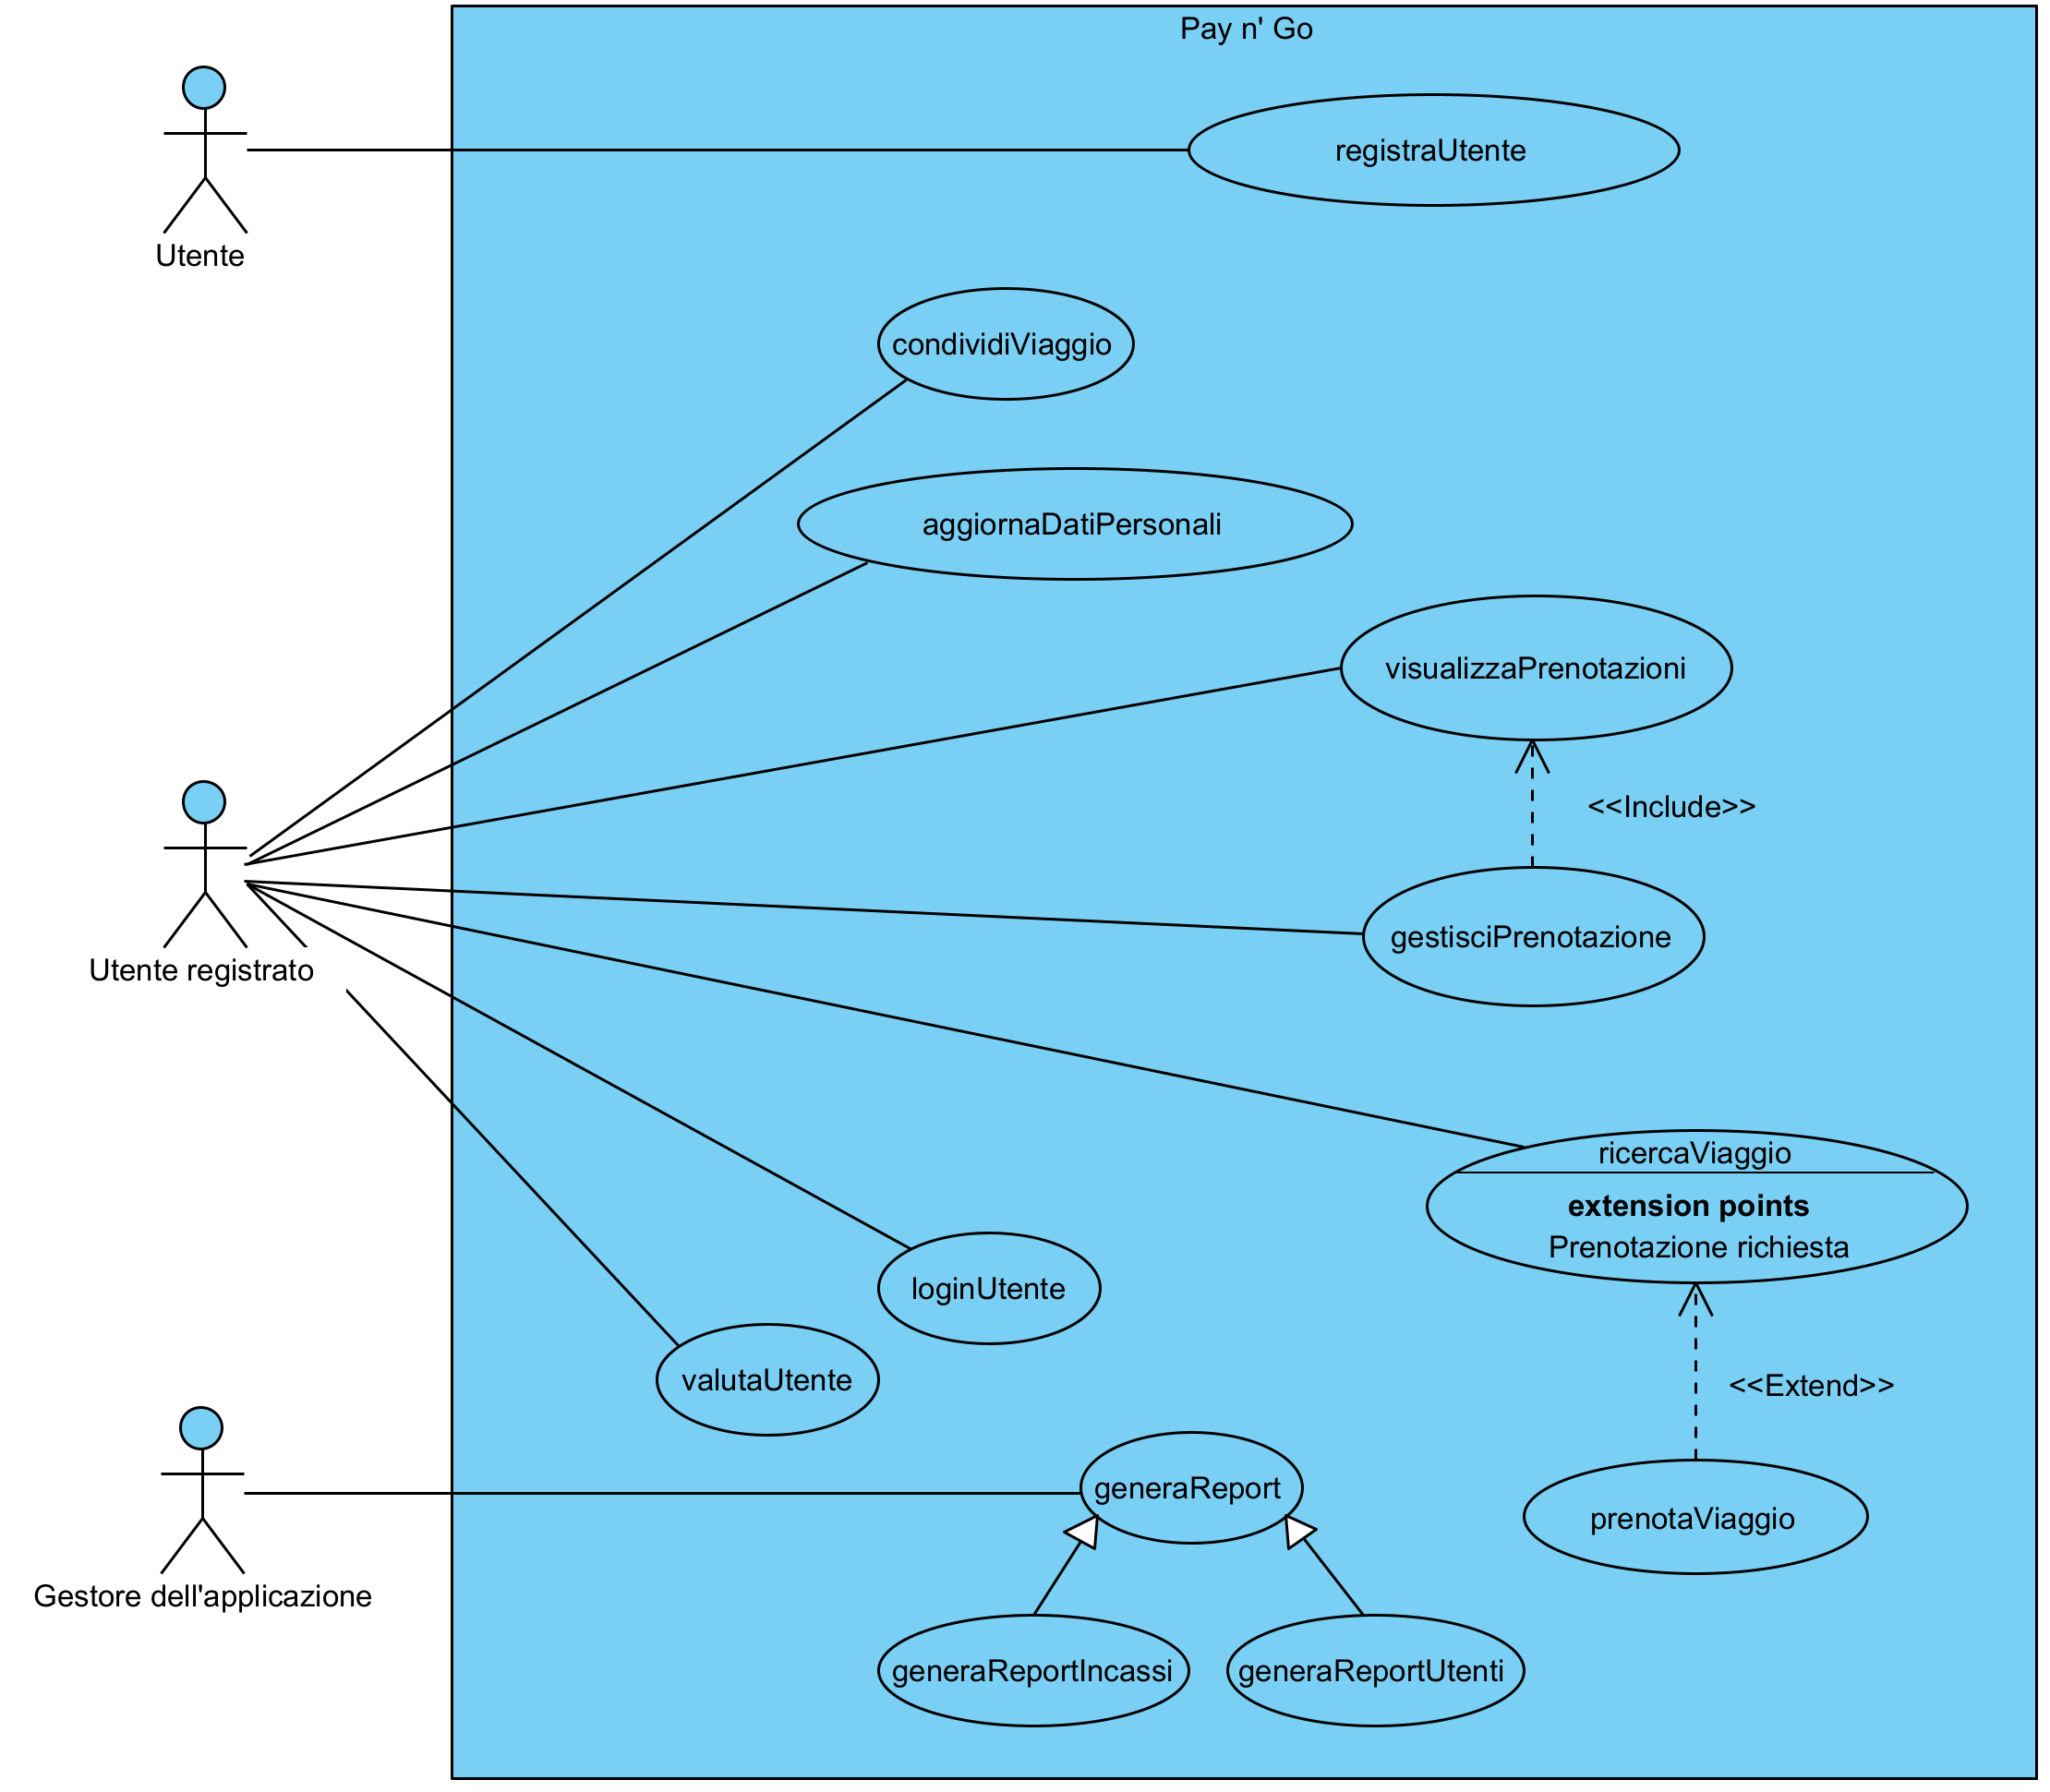
\includegraphics[scale=0.8]{img/diagrams/use_case_diagram.png}
    \caption{Diagramma dei casi d'uso}
\end{figure}

\subsubsection{Scenari}

\begin{flushleft}
\begin{usecase}
    \name{\textbf{Registrazione}}
    \actor{Utente}
    \udescription{Un Utente effettua la procedura di registrazione}
    \precondition{}
    \scenario{
        \item {Il caso d'uso ha inizio quando l'Utente richiede la registrazione al sistema}
        \item {Il sistema mostra all'Utente un'interfaccia in cui inserire i propri dati: nome, cognome, contatto telefonico, indirizzo email, password, tipo di automobile e numero di posti disponibili}
        \item {L'Utente inserisce i dati richiesti}
        \item {Il sistema controlla che l'Utente non sia già registrato}
        \begin{tabenum}
            \item {Se l'Utente è già registrato, il sistema mostra un opportuno messaggio di errore}
        \end{tabenum}
        \item {Il sistema memorizza i dati inseriti e notifica l'Utente dell'avvenuta registrazione}
    }
    \result{L'Utente è stato correttamente registrato}
    \extensions{}
    \exceptions{
        \item[3.a.]{L'Utente inserisce dati non validi}
        \begin{tabenum}
            \item[3.a.1.]{Il sistema segnala l'errore e chiede di inserire dei dati validi}
        \end{tabenum}
    }
\end{usecase}

\vspace{1cm}

\begin{usecase}
    \name{\textbf{CondividiViaggio}}
    \actor{Utente registrato}
    \udescription{Un Utente registrato condivide i dettagli di un viaggio}
    \precondition{L'Utente è stato autenticato dal sistema e ha un'automobile associata}
    \scenario{
        \item {Il caso d'uso ha inizio quando l'Utente registrato richiede al sistema di condividere i dettagli di un viaggio}
        \item {Il sistema mostra all'Utente registrato un'interfaccia in cui inserire le informazioni circa il viaggio: luogo di partenza, luogo di destinazione, data ed ora di partenza e contributo per le spese di viaggio}
        \item {L'Utente inserisce i dati richiesti}
        \item {Il sistema memorizza le informazioni del viaggio condiviso e notifica all'Utente l'avvenuta condivisione}
    }
    \result{L'Utente ha condiviso correttamente un viaggio}
    \extensions{}
    \exceptions{
        \item[3.a] L’Utente inserisce dati non validi
        \begin{tabenum}
            \item[3.a.1.]{Il sistema segnala l'errore e chiede di inserire dei dati validi}
        \end{tabenum}
    }
\end{usecase}

\vspace{1cm}

\begin{usecase}
    \name{\textbf{RicercaViaggio}}
    \actor{Utente registrato}
    \udescription{Un Utente registrato effettua la ricerca di un viaggio}
    \precondition{L'Utente è stato autenticato dal sistema}
    \scenario{
        \item {Il caso d'uso ha inizio quando l'Utente registrato richiede al sistema di ricercare un viaggio}
        \item {Il sistema mostra all'Utente registrato un'interfaccia in cui inserire i criteri di ricerca: luogo di partenza, luogo di destinazione e data ed ora di partenza}
        \item {L'Utente inserisce i dati richiesti}
        \item {Se il sistema trova uno o più viaggi}
        \begin{tabenum}
            \item {Per ogni viaggio trovato}
            \begin{tabenum}
              \item {Il sistema ne mostra i dettagli}
            \end{tabenum}
        \end{tabenum}
        \item {Altrimenti}
        \begin{tabenum}
            \item {Il sistema comunica all'Utente registrato che non sono stati trovati viaggi corrispondenti ai criteri di ricerca}
        \end{tabenum}
        \item {\textbf{Punto di estensione}: prenotazione richiesta}
    }
    \result{}
    \extensions{}
    \exceptions{
        \item[3.a] L’Utente inserisce dati non validi
        \begin{tabenum}
            \item[3.a.1.]{Il sistema segnala l'errore e chiede di inserire dei dati validi}
        \end{tabenum}
    }
\end{usecase}

\vspace{1cm}

\begin{usecase}
    \name{\textbf{Login}}
    \actor{Utente registrato}
    \udescription{Un Utente registrato effettua la procedura di login}
    \precondition{L'Utente non è autenticato dal sistema}
    \scenario{
        \item {Il caso d'uso ha inizio quando l'Utente registrato richiede di effettuare il login al sistema}
        \item {Il sistema mostra all'Utente registrato un'interfaccia in cui inserire i dati per effettuare il login: indirizzo email e password}
        \item {L'Utente inserisce i dati richiesti}
        \item {Il sistema verifica la validità dei dati inseriti}
        \item {Il sistema comunica all'Utente l'avvenuta autenticazione}
    }
    \result{L'Utente viene correttamente autenticato dal sistema}
    \extensions{
        
    }
    \exceptions{
        \item[4.a.] {L'Utente inserisce dati non validi}
        \begin{tabenum}
            \item[4.a.1.] {Il sistema segnala l'errore e chiede di inserire dei dati validi, negando l'autenticazione}
        \end{tabenum}
    }
\end{usecase}

\vspace{1cm}

\begin{usecase}
    \name{\textbf{ValutaUtente}}
    \actor{Utente registrato}
    \udescription{Un Utente registrato effettua una recensione di un altro Utente registrato}
    \precondition {L'Utente è autenticato dal sistema ed ha partecipato ad almeno un viaggio con l'Utente che intende recensire}
    \scenario{
        \item {Il caso d'uso inizia quando l'Utente registrato richiede di effettuare la valutazione di un determinato Utente registrato}
        \item {Il sistema richiede all'Utente registrato di selezionare l'Utente registrato che intende valutare}
        \item {Il sistema mostra all'Utente registrato un'interfaccia in cui inserire la valutazione dell'Utente registrato selezionato}
        \item {Il sistema memorizza la valutazione e notifica l'Utente registrato dell'esito dell'operazione}
    }
    \result{La valutazione è correttamente memorizzata}
    \extensions{}
    \exceptions{}
\end{usecase}

\vspace{1cm}

\begin{usecase}
    \name{\textbf{VisualizzaPrenotazioni}}
    \actor{Utente registrato}
    \udescription{Un Utente registrato visualizza le prenotazioni ai suoi viaggi condivisi}
    \precondition{L'Utente è autenticato dal sistema e deve aver condiviso almeno un viaggio}
    \scenario{
       \item {Il caso d'uso inizia quando l'Utente registrato richiede al sistema di visualizzare le prenotazioni ai suoi viaggi condivisi}
       \item {Il sistema mostra un'interfaccia in cui sono presenti le prenotazioni effettuate per ognuno dei viaggi condivisi dall'Utente registrato}
    }
    \result{Il sistema mostra le prenotazioni effettuate}
    \extensions{}
    \exceptions{}
\end{usecase}

\vspace{1cm}

\begin{usecase}
    \name{\textbf{GestisciPrenotazione}}
    \actor{Utente registrato}
    \udescription{Un Utente registrato gestisce una prenotazione, accettandola o rifiutandola}
    \precondition{L'Utente deve essere autenticato dal sistema e deve aver condiviso almeno un viaggio}
    \scenario{
        \item {include(VisualizzaPrenotazioni)}
        \item {L'Utente registrato seleziona una prenotazione che intende accettare o rifiutare}
        \item {Se l'Utente registrato accetta la prenotazione}
        \begin{tabenum}
            \item {Il sistema contrassegna la prenotazione come accettata}
        \end{tabenum}
        \item {Altrimenti}
        \begin{tabenum}
            \item {Il sistema cancella la prenotazione}
        \end{tabenum}
    }
    \result{La prenotazione è correttamente gestita}
    \extensions{}
    \exceptions{}
\end{usecase}

\vspace{1cm}

\begin{usecase}
    \name{\textbf{GeneraReportIncassi}}
    \actor{Gestore dell'applicazione}
    \udescription{Il Gestore dell'applicazione effettua la generazione del report sugli incassi}
    \precondition{Il Gestore dell'applicazione è correttamente autenticato}
    \scenario{
        \item {Il caso d'uso inizia quando il Gestore dell'applicazione richiede al sistema di generare il report sugli incassi}
        \item {Il sistema calcola l'incasso totale}
        \item {Il sistema mostra tramite un'interfaccia il report}
    }
    \result{Il sistema mostra il report sugli incassi}
    \extensions{}
    \exceptions{}
\end{usecase}

\vspace{1cm}

\begin{usecase}
    \name{\textbf{GeneraReportUtenti}}
    \actor{Gestore dell'applicazione}
    \udescription{Il Gestore dell'applicazione effettua la generazione del report sugli Utenti registrati}
    \precondition{Il Gestore dell'applicazione è correttamente autenticato}
    \scenario{
        \item {Il caso d'uso inizia quando il Gestore dell'applicazione richiede al sistema di generare il report sugli Utenti registrati}
        \item {Il sistema ottiene una lista di tutti gli Utenti registarti con le relative valutazioni}
        \item {Il sistema mostra tramite un'interfaccia il report}
    }
    \result{Il sistema mostra il report sugli Utenti registrati}
    \extensions{}
    \exceptions{}
\end{usecase}

\vspace{1cm}

\begin{usecase}
    \name{\textbf{PrenotaViaggio}}
    \actor{Utente registrato}
    \udescription{Un Utente registrato effettua la prenotazione di un posto per uno specifico viaggio}
    \precondition{L'Utente ha richiesto di prenotare un viaggio}
    \scenario{
       \item {include(RicercaViaggio)}
       \item {L'Utente seleziona il viaggio che intende prenotare}
       \item {L'Utente effettua la prenotazione del viaggio}
       \item {Il sistema genera un biglietto contenente ID della prenotazione, riferimento al guidatore, riferimento al passeggero ed il costo richiesto per il viaggio}
       \item {Il sistema memorizza il biglietto generato e notifica l'Utente dell'avvenuta prenotazione}
    }
    \result{La prenotazione è effettuata correttamente}
    \extensions{}
    \exceptions{}
\end{usecase}

\vspace{1cm}

\begin{usecase}
    \name{\textbf{AggiornaDatiPersonali}}
    \actor{Utente registrato}
    \udescription{L'Utente registrato aggiorna i suoi dati personali}
    \precondition{L'Utente registrato è correttamente autenticato}
    \scenario{
        \item {Il caso d'uso inizia quando l'Utente registrato richiede al sistema di aggiornare i propri dati personali}
        \item {Il sistema mostra all'Utente registrato un'interfaccia in cui inserire i dati personali aggiornati}
        \item {L'Utente registrato inserisce i nuovi dati}
        \item {Il sistema memorizza i dati aggiornati}
    }
    \result{I dati personali dell'Utente registrato sono stati corretamente aggiornati}
    \extensions{}
    \exceptions{
    \item[3.a.]{L'Utente inserisce dati non validi}
        \begin{tabenum}
            \item[3.a.1.]{Il sistema segnala l'errore e chiede di inserire dei dati validi}
        \end{tabenum}}
\end{usecase}


\end{flushleft}

\subsection{Diagramma delle classi}

\begin{figure}[H]
    \centering
    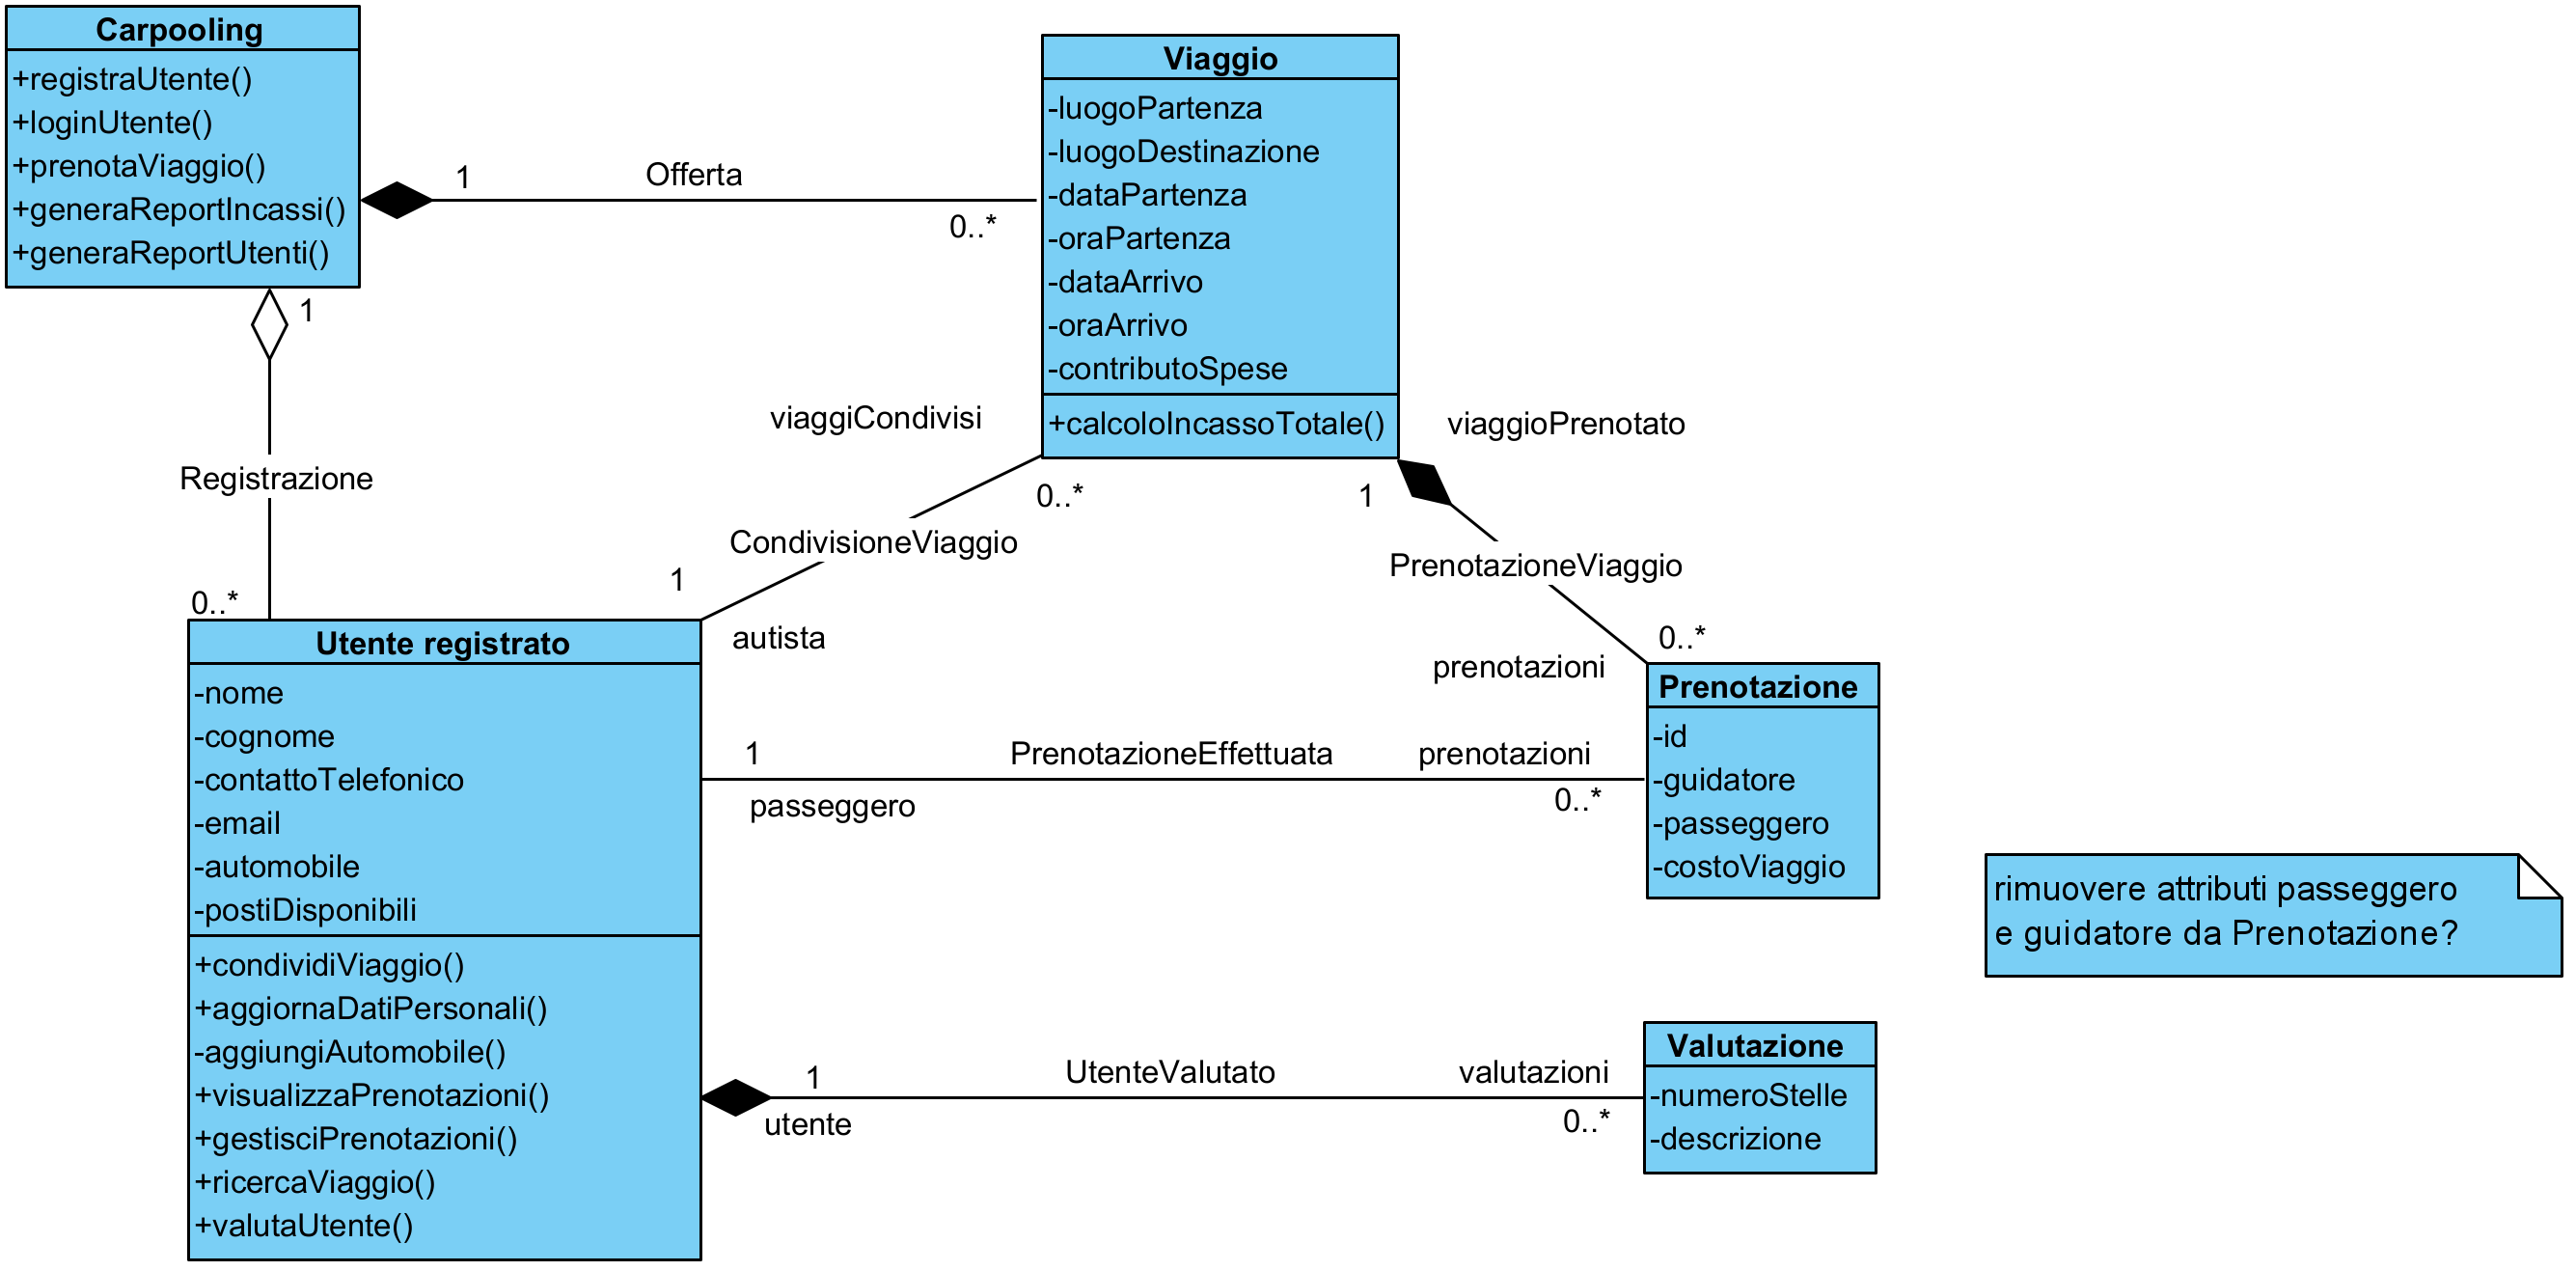
\includegraphics[scale=0.8]{img/diagrams/class_diagram.png}
    \caption{Diagramma delle classi}
\end{figure}

Questo diagramma consente una visualizzazione di alto livello della struttura delle varie classi che compongono il sistema. Esso andrà successivamente raffinato con una più dettagliata specifica di ogni classe.

\section {DOMANDE}

\begin{itemize}
    \item Controlla Sequence di CondividiViaggio forse troppo complesso
    \item AggiungiAutomobile potrebbe essere inutile. Non sarebbe meglio come scenario alternativo?
    \item Login forse è meglio che abbia come attore principale l'Utente per gestire il caso in cui un utente non registrato provi a fare login. Ma soprattutto, come cazzo va fatto che so due cose del dioporco
\end{itemize}

\section {TODO}

\begin{itemize}
    \item {Aggiusta diagramma CD "registrazione" a "registraUtente"}
    \item {Aggiunta classe "Valutazione", sicuramente servono dei metodi }
\end{itemize}

\end{document}

